\begin{enumerate}


\item Students of a school are taken to a railway museum to learn about railways heritage and its history\\
	\begin{figure}[h!]
		\centering
		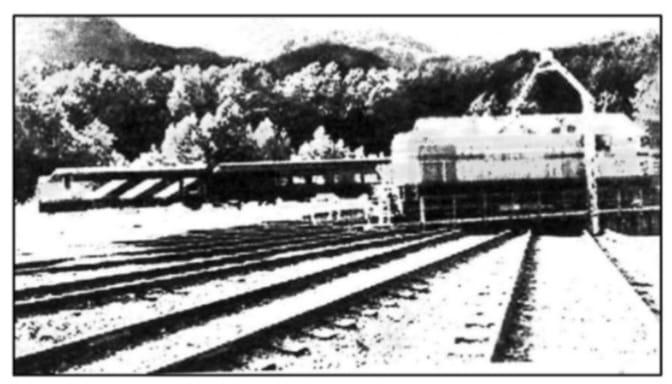
\includegraphics[width=0.8\textwidth]{figs/fig1.jpg}
		\label{fig:image1}
	\end{figure}
	An exhibt in the museum depicted many rail lines on the tack near the railway station. let $L$ be the set of all ral lines on the railwa track and $R$ be the relation on $L$ defined by\\
		$R$={$(l_{1},l_{2}):l_{1} $is parallel to $l_{2}$}\\
	On the basis of the above information, answer the following questions:
\begin{enumerate}
\item Find whether the relation $R$ is symmetric or not.

\item Find whether the relation $R$ is transitive or not.

\item If one of the rail lines on the railway track is represented by the equation $y = 3x + 2$ then find the set of rail lines in $R$ related to it.

\end{enumerate}
\item Let $S$ be the relation defined by $S$ = {$( l_{1},l_{2}):l_{1}$ is perpendicular to $l_{2}$} check whether the relation $S$ is symmetric and transitive.



\end{enumerate}
